\documentclass[12pt]{article}

\usepackage{pst-all}
\usepackage{demo}

\let\orgheader\adviheader
\def\adviheader{\orgheader\advibg{image=adviback.ppm}}

%Didier's flashy macro
\def \flash #1{\let \do\leflash \do #1\relax}
\def \leflash #1{\ifx #1\relax \def \do{}\else \def \do {#1\adviwait[1]\leflash}\fi \do}

\advibg[global]{image=adviback.ppm}
\begin{document}
\newpage

\subsection* {{\ActiveDVI} is:}

A {\bf DVI} presenter (based on {\tt mldvi} by Alexandre Miquel for
the DVI rendering engine)

\bigskip

\noindent
\advitransbox{wipe,from=left}{%
\begin{minipage}{\textwidth}
\begin {itemize}
\item[+] dvips
  \textcolor{c1}{c}%
  \textcolor{c2}{o}%
  \textcolor{c3}{l}%
  \textcolor{c4}{o}%
  \textcolor{c5}{u}%
  \textcolor{c6}{r}
  extension (by Alexandre Miquel)
\item[+] bitmap inclusion with cache (by Jun Furuse)
\item[+] GPIC specials (by Xavier Leroy)
\item[+] Postscript specials (by Didier R{\'{e}}my)
\item[+] hyperrefs (by Didier R{\'{e}}my)
\item[+] active anchors with annotated texts (by Didier R{\'{e}}my)
\item[+] animations and transitions (Jun Furuse and Didier R\'emy)
\item[+] swallowed applications (Jun Furuse and Pierre Weis)
\item[+] and other gadgets...
\end {itemize}
\end{minipage}}

\newpage
\advitransition{wipe}

\subsection*{Presentation macros}
\noindent
\verb|\adviwait|\\
\verb|\advirecord{|{\em text\ }\verb|}|, 
\verb|\adviplay|\\
\verb|\begin{advirecording}|
{\em text}
\verb|\end{advirecording}|

\bigskip

\noindent
Press any key to launch  the demo:
\adviwait

\advitransition{none} % we must reset the transition
\noindent
\verb+\adviwait[+{\em time}\verb+]+ counts down for you:
3\ldots\adviwait[1]2\ldots\adviwait[1]1\ldots\adviwait[1]\textcolor{red}{GO!}

\vfill

\noindent
\begin{tabular}{l}
\advirecord{H}{Hamlet}: Do you see yonder cloud that's almost in shape of a \advirecord{C}{\rnode{CN1}{camel}}?\\
\advirecord{P}{Plonius}: By th'mass, and 'tis like a \advirecord{C}{\rnode{CN2}{camel}}, indeed\\
\advirecord{H}{Hamlet}: Methinks it is like a \advirecord{W}{\rnode{CN3}{weasel}}\\
\advirecord{P}{Plonius}: It is back'd like a \advirecord{W}{\rnode{CN4}{weasel}}\\
\advirecord{H}{Hamlet}: Or like a \advirecord{W2}{\rnode{CN5}{whale}}?\\
\advirecord{P}{Plonius}: Very like a \advirecord{W2}{\rnode{CN6}{whale}}.
\end{tabular}\\
\noindent
{\small \hfill (\advirecord{H}{Hamlet}  by William Shakespeare, Act III, scene 3.)}

\begin{enumerate}
\item Who are they ? \advirecord{H}{Hamlet} and \advirecord{P}{Plonius}.
\advirecord{Q2}{\item What do they say ? \advirecord{C}{Camel}, \advirecord{W}{weasel} and \advirecord{W2}{whale}.}
\advirecord{Q3}{\item And what do they actually see ? \advirecord{C2}{Of course, \rnode{CN0}{\textcolor{red}{CAML!}}}}
\end{enumerate}

\adviwait
\adviplay[red]{H}
\adviwait
\adviplay[black]{H}
\adviplay[red]{P}
\adviwait
\adviplay[black]{P}
\adviplay{Q2}
\adviwait
\adviplay[red]{C}
\adviwait
\adviplay[black]{C}
\adviplay[red]{W}
\adviwait
\adviplay[black]{W}
\adviplay[red]{W2}
\adviwait
\adviplay[black]{W2}
\adviplay{Q3}
\adviwait
\adviplay{C2}
\nccurve[linecolor=red,linewidth=3pt,angleA=0,angleB=280]{->}{CN0}{CN1}
\nccurve[linecolor=red,linewidth=3pt,angleA=0,angleB=350]{->}{CN0}{CN2}
\nccurve[linecolor=red,linewidth=3pt,angleA=0,angleB=350]{->}{CN0}{CN3}
\nccurve[linecolor=red,linewidth=3pt,angleA=0,angleB=355]{->}{CN0}{CN4}
\nccurve[linecolor=red,linewidth=3pt,angleA=0,angleB=0]{->}{CN0}{CN5}
\nccurve[linecolor=red,linewidth=3pt,angleA=0,angleB=0]{->}{CN0}{CN6}
\vfill

\vfill

\newpage
\advitransition{wipe}

\subsection*{EPS Bitmap inclusion}
\begin{center}
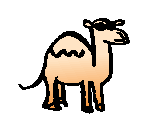
\includegraphics[width=0.15\textwidth,height=0.15\textwidth]{../tex/caml.eps}
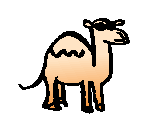
\includegraphics[width=0.3\textwidth,height=0.15\textwidth]{../tex/caml.eps}  
\end{center}

\subsection*{GPIC: Pictures for \TeX}

\def\showgraph{%
  \par\medskip\centerline{\raise 1em\box\graph}\bigskip\noindent\ignorespaces}
This chapter is contributed by F. de~Dinechin with assistance of C.
Daramy-Loirat and D. Defour.

\section*{Introduction}
This chapter describes the implementations of sine, cosine and
tangent, as they share much of their code. The proof sketch below is
supported by the Maple script \texttt{maple/trigo.mpl} and the Gappa
scripts \texttt{gappa/trigoSinCosCase3.gappa} and
\texttt{gappa/trigoTanCase2.gappa} of the \crlibm\ distribution. These scripts 
implement the computations of error bounds and validity bounds for the
various algorithmic paths described here.

\section{Overview of the algorithms}

\subsection{Exceptional cases}

The three trigonometric functions return NaN for infinite and NaN
arguments, and are defined otherwise. 

An argument based on continued fractions to find the worst cases for
range reduction may also be used to show that the sine and cosine of a
floating-point number outside of $[-1,1]$ is always larger than
$2^{-150}$, and therefore never flushes to zero nor to subnormal (see
\cite{Muller97} p. 151 and following). Therefore
$\tan(x)=\sin(x)/\cos(x)$ also remains larger than $2^{-150}$.

This has two important consequences:

\begin{itemize}
\item as the output a trigonometric function is never a subnormal except for
  inputs around zero (for which the value to return is trivial
  anyway), we can safely use the rounding tests from Section
  \ref{section:testrounding} p.~\pageref{section:testrounding}.

\item as the cosine never flushes to zero, the tangent of a
  floating-point number is never an infinity, and does not even come
  close, so again we may safely use the rounding tests from Section
  \ref{section:testrounding}.
\end{itemize}

For very small arguments,
\begin{itemize}
\item $\sin(x) = x-x^3/6 + O(x^5) = x(1-x^2/6) + O(x^5)$ where
  $O(x^5)$ has the sign of $x$. Therefore $\sin(x)$ is rounded to $x$
  or one of its floating-point neighbours as soon as $|x|<2^{-26}$.
\item $\cos(x) = 1-x^2/2 + O(x^4)$ where $O(x^4)$ is positive.
  Therefore $\cos(x)$ is rounded to $1$ in RN and RU mode if
  $x<\sqrt{2^{-53}}$. In RD and RZ modes, we have $\cos(0)=1$ and
  $\cos(x)=1-2^{-53}$ for $|x|<2^{-26}$.
\item $\tan(x) = x+x^3/3 + O(x^5) = x(1+x^2/3) + O(x^5)$ where
  $O(x^5)$ has the sign of $x$. Therefore $\tan(x)$ is rounded to $x$
  or one of its neighbours for all the rounding  modes if $|x|<2^{-27}$.
\end{itemize}


\subsection{Range reduction}

Most implementations of the trigonometric functions have two steps of range reduction: 
\begin{itemize}
\item first the input number $x$ is reduced to $y\in
  [-\frac{\pi}{4}, \frac{\pi}{4}]$, with reconstruction using periodicity and
  symmetry properties,
\item then the reduced argument is further broken down as $y=a+z$,
  with reconstruction using the formula for $\sin(a+z)$ and
  $\cos(a+z)$, using tabulated values of $\sin(a)$ and
  $\cos(a)$
\end{itemize}

We chose to implement range reduction in one step only, which
computes an integer $k$ and a reduced argument y such that

\begin{equation}
  x = k\frac{\pi}{256} + y\label{eq:trigoargred}
\end{equation}
where $k$ is an integer and  $ |y| \leq {\pi}/{512}$.
This step computes $y$ as a double-double: $y\approx y_h+y_l$. 

In the following we note $$a=k\pi/256.$$ 

Then we read off a table 

$$sa_h+sa_l \approx sin(a)$$
$$ca_h+ca_l \approx cos(a)$$

Only 64 quadruples $(sa_h,sa_l,ca_h,ca_l)$ are tabulated (amounting to
$64\times 8 \times 4 = 2048$ bytes), the rest is obtained by
periodicity and symmetry, implemented as masks and integer operations
on the integer $k$. For instance,  $a \mod 2\pi$ is implemented by $k \mod 512$,
$\pi/2-a$ is implemented as $128-k$, etc.



Then we use the reconstruction steps:

\begin{equation}        
  \sin(x) = \sin(a + y) =  \cos(a) \sin(y) +  \sin(a) \cos(y) 
  \label{eq:sinapy}
\end{equation}

\begin{equation}
  \cos(x) = \cos(a + y) = \cos(a) \cos(y) -  \sin(a) \sin(y) 
  \label{eq:cosapy}
\end{equation}

\begin{equation} 
  tan(x) = \frac{\sin(x)}{\cos(x)} 
  \label{eq:tanapy}
\end{equation}


\subsection{Polynomial evaluation}


To implement the previous equations, $\cos(y)$ and $\sin(y)$ are
computed as unevaluated $1+t_c$ and $(y_h+y_l)(1+t_s)$ respectively,
where $t_c$ and $t_s$ are doubles computed using a polynomial
approximation of small degree:

\begin{itemize}
\item $t_s = y^2(s_3 + y^2(s_5 + y^2s_7)))$ with $s3$, $s5$ and
$s7$ the Taylor coefficients.
\item $t_c = y^2(c_2 + y^2(c_4 + y^2c_6))$ with $c2$, $c4$ and $c6$ the
Taylor coefficients (or a more accurate minimax approximation).
\end{itemize}



\subsection{Reconstruction}

\subsubsection{Sine}
According to equation (\ref{eq:sinapy}), we have to compute: 
 \begin{eqnarray*}
  \sin(a+y) &=& \sin(a) \cos(y)  + \cos(a)\sin(y)  \\
  & \approx& (sa_h+sa_l)(1+t_c) + (ca_h+ca_l)(y_h+y_l)(1+t_s)
\end{eqnarray*}


Figure~\ref{fig:sine-reconstruction} shows the worst-case respective
orders of magnitude of the terms of this sum. The terms completely to the
right of the vertical bar will be neglected, and a bound on the
error thus entailed is computed in the following. Note that the term
$ca_hy_h$ has to be computed exactly by a Mul12.

Finally the reconstruction consists of adding together the lower-order
terms in increasing order of magnitude, and computing the
double-double result by an Add12.

\begin{figure}[htbp]    
  \begin{center}
    \small
    \setlength{\unitlength}{3ex}
      \framebox{
        \begin{picture}(22,9)(-3,-4.2)
          \put(9.5,4){\line(0,-1){8}}  %\put(9,4){$\epsilon$}
          
          \put(4,3.2){$sa_h$} \put(0.05,3){\framebox(7.9,0.7){}}
          \put(12,3.2){$sa_l$}  \put(8.05,3){\framebox(7.9,0.7){}}
          
          \put(6,2.2){$sa_ht_c$} \put(2.05,2){\framebox(7.9,0.7){}}
          \put(14,2.2){$sa_lt_c$}  \put(10.05,2){\framebox(7.9,0.7){}}

          \put(4.5,1.2){$ca_hy_h$} \put(0.55,1){\framebox(7.9,0.7){}}
          \put(12.5,1.2){$ca_hy_h$}  \put(8.55,1){\framebox(7.9,0.7){}}

          \put(11.5,0.2){$ca_hy_l $}  \put(7.55,0){\framebox(7.9,0.7){}}
          \put(11.5,-0.8){$ca_ly_h $}  \put(7.55,-1){\framebox(7.9,0.7){}}

         \put(6.5,-1.8){$ca_hy_ht_s$} \put(2.55,-2){\framebox(7.9,0.7){}}
         \put(13.5,-2.8){$ca_hy_lt_s $}  \put(9.55,-3){\framebox(7.9,0.7){}}
         \put(13.5,-3.8){$ca_ly_ht_s $}  \put(9.55,-4){\framebox(7.9,0.7){}}
        
       \end{picture}
     }
   \end{center}
   \caption{The sine reconstruction}
   \label{fig:sine-reconstruction}
 \end{figure}
 
 

\subsubsection{Cosine}
According to equation (\ref{eq:cosapy}), we have to compute in double-double precision:
 \begin{eqnarray*}
  \cos(a+y) &=& \cos(a) \cos(y)  - \sin(a)\sin(y)  \\
  & \approx& (ca_h+ca_l)(1+t_c) - (sa_h+sa_l)(y_h+y_l)(1+t_s)
\end{eqnarray*}

This is similar to the case of the sine, and the respective orders of
magnitude are given by Figure~\ref{fig:sine-reconstruction}.

\begin{figure}[htbp]
  \begin{center}
    \small \setlength{\unitlength}{3ex} \framebox{
      \begin{picture}(22,9)(-3,-4.2)
        \put(9.5,4){\line(0,-1){8}}
%        \put(9,4){$\epsilon$}
  
        \put(4,3.2){$ca_h$} \put(0.05,3){\framebox(7.9,0.7){}}
        \put(12,3.2){$ca_l$}  \put(8.05,3){\framebox(7.9,0.7){}}

        \put(6,2.2){$ca_ht_c$} \put(2.05,2){\framebox(7.9,0.7){}}
        \put(14,2.2){$ca_lt_c$}  \put(10.05,2){\framebox(7.9,0.7){}}

        \put(4.5,1.2){$-sa_hy_h$} \put(0.55,1){\framebox(7.9,0.7){}}
        \put(12.5,1.2){$-sa_hy_h$}  \put(8.55,1){\framebox(7.9,0.7){}}

        \put(11.5,0.2){$-sa_hy_l $}  \put(7.55,0){\framebox(7.9,0.7){}}
        \put(11.5,-0.8){$-sa_ly_h $}  \put(7.55,-1){\framebox(7.9,0.7){}}

        \put(6.5,-1.8){$-sa_hy_ht_s$} \put(2.55,-2){\framebox(7.9,0.7){}}
        \put(13.5,-2.8){$-sa_hy_lt_s $}  \put(9.55,-3){\framebox(7.9,0.7){}}
        \put(13.5,-3.8){$-sa_ly_ht_s $}  \put(9.55,-4){\framebox(7.9,0.7){}}
 
        \end{picture}
      }
    \end{center}\centering
    
    \caption{The cosine reconstruction}
    \label{fig:cosine-reconstruction}
  \end{figure}


\subsubsection{Tangent}

The tangent is obtained by the division of the sine by the cosine,
using the \texttt{Div22} procedure which is accurate to  $2^{-104}$.


\subsection{Precision of this scheme}

As we have $|y|<2^{-7}$, this scheme computes these functions
accurately to roughly $2^{53+13}$ bits, so these first steps are very
accurate. 
 

\subsection{Organisation of the code}


The code for range reduction is shared by the three
trigonometric functions. It is detailed and proven in
Section~\ref{trigo:argred}.

Then there are four procedures (currently implemented as macros for
efficiency), respectively called \texttt{DoSinZero},
\texttt{DoCosZero}, \texttt{DoSinNotZero} and \texttt{DoCosNotZero}
which do the actual computation after range reduction as per
Figures~\ref{fig:sine-reconstruction} and
\ref{fig:cosine-reconstruction}. The tangent function is computed by
dividing the sine by the cosine. These procedures are studied in
section \ref{trigo:auxiliary}.

Finally, each of the three trigonometric functions comes in four
variants for the four rounding modes. These four variants differ in
the beginning (special cases) and in the end (rounding), but share the
bulk of the computation. The shared computation is called
\verb!compute_trig_with_argred!.




\section{Details of range reduction
\label{trigo:argred}}

\subsection{Which accuracy do we need for range reduction?}

The additive reduction consists in adding or removing $N$ times a
certain constant $C$ from the input argument. For trigonometric
function this constant is usually equal to $\pi/2$ or $\pi/4$, in our
case it is $\pi/128$. A naive range reduction based on
machine precision for trigonometric function would be implemented as :

\begin{equation}
\begin{array}{rcl}
k    &=&  \lfloor \frac{x}{C} \rfloor \\
x^*  &=&  x-kC. \\
\end{array}
\label{chap6:eqn:rangereduction}
\end{equation}

Obviously, this subtraction cancels all the bits common to $x$ and $kC$:
\begin{itemize}
\item The absolute accuracy of $x^*$ with respect to the exact value
  of $x-kC$ depends only on the precision used to compute the subtraction
  and the product in $x-kC$ ($x$ is considered exact as it is the
  input to the function).

\item However, the relative accuracy of $x^*$ with respect to the
  exact value of $x-kC$ also depends on this exact value. For a given
  precision of the operations used in computing $x-kC$, the closer $x$
  to $kC$, the smaller the exact value of $x-kC$, and the worse the
  relative accuracy (or, in less formal terms, the more bits of the
  results are lost to cancellation).
\end{itemize}

As the theorems for correct rounding of
Section~\ref{section:testrounding} p.~\pageref{section:testrounding}
depend on the relative accuracy of the evaluation (and therefore on
the relative accuracy of the reduced argument), we have to prove
bounds on the relative accuracy of range reduction.

Formulated in simpler terms, how many bits can be lost in the
subtraction $x-kC$ ? This number is related to the knowledge of the
closest input number $x$ to a multiple of $C$. There exists an
algorithm due to Kahan/Douglas and based on continued fraction to
compute this number and therefore the number of bit lost (see
\cite{Muller97} p. 151 and following).  We used a Maple version from
\cite{Muller97} to determine than up to 62 bits may be cancelled
during range reduction for a ieee double precision number. This Maple
procedure is implemented as function
\texttt{WorstCaseForAdditiveRangeReduction} in
\texttt{maple/common-procedures.mpl}.

One advantage of having $C=\pi/128$, however, is that this is only a
concern when $x$ is close to a multiple of $\pi/2$ (that is, $k \mod
128=0$): in the other cases (i.e. in the general, most frequent case)
the reconstruction will add some tabulated non-zero value, so the
error to consider in the range reduction is the absolute error.  Only
in the cases when $k \mod 128=0$ do we need to have 62 extra bits to
compute with. This is ensured by using a slower, more accurate range
reduction. As a compensation, in this case when $k \mod 128=0$, there
is no table to read and no reconstruction to perform: a simple
polynomial approximation to the function suffices.



\subsection{Details of the used scheme}

We have 4 possible range reductions, depending on the magnitude of the
input number (and the previous considerations):

\begin{itemize}
\item Cody and Waite with 2 constants (the fastest),
\item Cody and Waite with 3 constants (almost as fast),
\item Cody and Waite with 3 constants in double-double and $k$ a
  64-bit int, and 
\item Payne and Hanek, implemented in SCS (the slowest).
\end{itemize}
Each of these range reductions except Payne and Hanek is valid for $x$
smaller than some bound. The computation of these bounds is detailed
below.

Section \ref{trigo:structargred} details the organization of this
multi-level range reduction, and is followed by a detailed proof of
each level.



\subsection{Structure of the range reduction
  \label{trigo:structargred}} The complete code is detailed below. To
provide a complete picture to the reader it actually also includes the
reconstruction.

\begin{lstlisting}[caption={Multilevel range reduction \label{lst:trig:argred}},firstnumber=1]
struct rrinfo_s {double rh; double rl; double x; int absxhi; int function;} ;
typedef struct rrinfo_s rrinfo;
#define changesign function /* saves one int in the rrinfo structure */

static void ComputeTrigWithArgred(rrinfo *rri){ 
  double sah,sal,cah,cal, yh, yl, yh2, ts,tc, kd; 
  double kch_h,kch_l, kcm_h,kcm_l, th, tl,sh,sl,ch,cl;
  int k, quadrant, index;
  long long int kl;

  if  (rri->absxhi < XMAX_CODY_WAITE_3) {
    /* Compute k, deduce the table index and the quadrant */
    DOUBLE2INT(k, rri->x * INV_PIO256);
    kd = (double) k;
    quadrant = (k>>7)&3;      
    index=(k&127)<<2;
    if((index == 0)) { 
      /* Here a large cancellation on yh+yl would be a problem, so use double-double RR */
      /* all this is exact */
      Mul12(&kch_h, &kch_l,   kd, RR_DD_MCH);
      Mul12(&kcm_h, &kcm_l,   kd, RR_DD_MCM);
      Add12 (th,tl,  kch_l, kcm_h) ;
      /* only rounding error in the last multiplication and addition */ 
      Add22 (&yh, &yl,    (rri->x + kch_h) , (kcm_l - kd*RR_DD_CL),   th, tl) ;
      goto computeZero;
    } 
    else {      
      /* index <> 0, don't worry about cancellations on yh+yl */
      if (rri->absxhi < XMAX_CODY_WAITE_2) {
	/* CW 2: all this is exact but the rightmost multiplication */
	Add12 (yh,yl,  (rri->x - kd*RR_CW2_CH),  (kd*RR_CW2_MCL) ) ; 
      }
      else { 
	/* CW 3: all this is exact but the rightmost multiplication */
	Add12Cond(yh,yl,  (rri->x - kd*RR_CW3_CH) -  kd*RR_CW3_CM,   kd*RR_CW3_MCL);
      }
    }
    goto computeNotZero;
  }

  else if ( rri->absxhi < XMAX_DDRR ) {
    /* x sufficiently small for a Cody and Waite in double-double */
    DOUBLE2LONGINT(kl, rri->x*INV_PIO256);
    kd=(double)kl;
    quadrant = (kl>>7)&3;
    index=(kl&127)<<2;
    if(index == 0) { 
      /* Here again a large cancellation on yh+yl would be a problem, 
	 so we do the accurate range reduction */
      RangeReductionSCS();   /*recomputes k, index, quadrant, and yh and yl*/
      /* Now it may happen that the new k differs by 1 of kl, so check that */
      if(index==0)   /* no surprise */
	goto computeZero; 
      else 
	goto computeNotZero;
    }
    else {   /*  index<>0 : double-double range reduction*/
      /* all this is exact */
      Mul12(&kch_h, &kch_l,   kd, RR_DD_MCH);
      Mul12(&kcm_h, &kcm_l,   kd, RR_DD_MCM);
      Add12 (th,tl,  kch_l, kcm_h) ;
      /* only rounding error in the last multiplication and addition */ 
      Add22 (&yh, &yl,    (rri->x + kch_h) , (kcm_l - kd*RR_DD_CL),   th, tl) ;
      goto computeNotZero;
    }
  } /* closes if ( absxhi < XMAX_DDRR ) */ 

  else {
    /* Worst case : x very large, sin(x) probably meaningless, we return
       correct rounding but do't mind taking time for it */
    RangeReductionSCS(); 
    quadrant = (k>>7)&3;                                       
    if(index == 0)
      goto computeZero;
    else 
      goto computeNotZero;
  }


 computeZero:
  switch(rri->function) {
 
  case SIN: 
    if (quadrant&1)
      DoCosZero(&rri->rh, &rri->rl);
    else 
      DoSinZero(&rri->rh, &rri->rl);
    rri->changesign=(quadrant==2)||(quadrant==3);
    return;
    
  case COS: 
    if (quadrant&1)
      DoSinZero(&rri->rh, &rri->rl);
    else 
      DoCosZero(&rri->rh, &rri->rl);
    rri->changesign= (quadrant==1)||(quadrant==2);
    return;

  case TAN: 
    rri->changesign = quadrant&1;
    if (quadrant&1) {
      DoSinZero(&ch, &cl);
      DoCosZero(&sh, &sl);
    } else {
      DoSinZero(&sh, &sl);
      DoCosZero(&ch, &cl);
    }
    Div22(&rri->rh, &rri->rl, sh, sl, ch, cl);
    return;
  }
  
 computeNotZero:
  if(index<=(64<<2)) {                                    
    sah=sincosTable[index+0].d; /* sin(a), high part */   
    sal=sincosTable[index+1].d; /* sin(a), low part  */   
    cah=sincosTable[index+2].d; /* cos(a), high part */   
    cal=sincosTable[index+3].d; /* cos(a), low part  */   
  }else { /* cah <= sah */                                
    index=(128<<2) - index;                               
    cah=sincosTable[index+0].d; /* cos(a), high part */   
    cal=sincosTable[index+1].d; /* cos(a), low part  */   
    sah=sincosTable[index+2].d; /* sin(a), high part */   
    sal=sincosTable[index+3].d; /* sin(a), low part  */   
  }                                                       
  yh2 = yh*yh ;
  ts = yh2 * (s3.d + yh2*(s5.d + yh2*s7.d));	
  tc = yh2 * (c2.d + yh2*(c4.d + yh2*c6.d ));	
  switch(rri->function) {

  case SIN: 
    if (quadrant&1)   
      DoCosNotZero(&rri->rh, &rri->rl);
    else 
      DoSinNotZero(&rri->rh, &rri->rl);
    rri->changesign=(quadrant==2)||(quadrant==3);
    return;

  case COS: 
    if (quadrant&1)   
      DoSinNotZero(&rri->rh, &rri->rl);
    else 
      DoCosNotZero(&rri->rh, &rri->rl);
    rri->changesign=(quadrant==1)||(quadrant==2);
    return;

  case TAN: 
    rri->changesign = quadrant&1;
    if (quadrant&1) {
      DoSinNotZero(&ch, &cl);
      DoCosNotZero(&sh, &sl);
    } else {
      DoSinNotZero(&sh, &sl);
      DoCosNotZero(&ch, &cl);
    }
    Div22(&rri->rh, &rri->rl, sh, sl, ch, cl);
    return;
  }
}
\end{lstlisting}
 

Here are some comments on the structure of this code (the details on
actual range reduction come in the following sections).

\begin{itemize}
\item The DOUBLETOINT macro at line 13 is called only if
  $x<\verb!XMAX_CODY_WAITE_3!$ (line 11). This constant is defined  (see
  Listing~\ref{trigo:lst:cw3maple} below) such
  that the conditions for this macro to work (see
  Section~\ref{sec:double2int}) are fullfilled. 

\item Similarly for the DOUBLETOLONGINT macro (see
  Section~\ref{sec:double2longint}) at line 43, which is called for
  inputs smaller than \verb!XMAX_DDR! defined in Listing
  \ref{trigo:lst:cwddrmaple} below.

\item There is one subtlety at lines 51 and following. There we take
  the decision of computing a more accurate range reduction depending
  on the value of $\mathit{index}=k\mod 256$. However, in the case
  when $x\times\frac{256}{\pi}$ is very close to the middle between
  two integers, it may happen (very rarely) that the value of $k\mod
  256$ computed by this second range reduction differs from the first
  by $\pm 1$. In such cases, both values will provide different but
  equally valid reduced arguments, but we have to ensure that $k$ and
  the reduced value match, hence the test line 52.
\end{itemize}



\subsection{Cody and Waite range reduction with two constants}

Here we split $C$ into two floating-point constants $C_h$ and $C_l$
such that $C_h$ holds 21 bits of the mantissa of $C$ (the rest being
zeroes), and $C_l=\round(C-C_h)$.  The following gives the
Maple code that computes these constants, and then computes the
bound on which this range reduction is valid.

\begin{lstlisting}[caption={Maple script for computing constants for Cody and Waite 2},
  firstnumber=1,  language={sh}, numbers=none]% of course it's maple
%Skip a line here, I don't know why, otherwise latex eats the first line

bitsCh_0:=32:  # ensures at least 53+11 bits

# 1/2 <= C/2^(expC+1) <1
Ch:= round(evalf(  C * 2^(bitsCh_0-expC-1))) / (2^(bitsCh_0-expC-1)):
# recompute bitsCh in case we are lucky (and we are for bitsCh_0=32)
bitsCh:=1+log2(op(2,ieeedouble(Ch)[3])) :  # this means the log of the denominator

Cl:=nearest(C - Ch):
# Cody and Waite range reduction will work for |k|<kmax_cw2
kmax_cw2:=2^(53-bitsCh):

# The constants to move to the .h file
RR_CW2_CH := Ch:
RR_CW2_MCL := -Cl:
XMAX_CODY_WAITE_2 := nearest(kmax_cw2*C):
\end{lstlisting}

The C code that performs the reduction in this case is the following:

\begin{lstlisting}[caption={Cody and Waite range reduction with two
    constants},firstnumber=31]
	Add12 (yh,yl,  (x - kd*RR_CW2_CH),  (kd*RR_CW2_MCL) ) ;
\end{lstlisting}

Here only the rightmost multiplication involving a rounding: 
\begin{itemize}
\item The multiplication $\mathrm{kd}\otimes \mathrm{RR\_CW2\_CH}$ is
  exact because $kd$ is a small integer and $\mathrm{RR\_CW2\_CH}$
  has enough zeroes in the mantissa.
\item The subtraction is exact thanks to Sterbenz Lemma.
\item The \texttt{Add12} procedure is exact.
\end{itemize}

The following Maple code thus computes the maximum absolute error on
the reduced argument (with respect to the ideal reduced argument) in
this case.
\begin{lstlisting}[caption={Maple script for computing absolute error for Cody and Waite 2},
  firstnumber=1,  language={sh}, numbers=none]% of course it's maple

delta_repr_C_cw2   := abs(C-Ch-Cl);
delta_round_cw2    := kmax_cw2 * 1/2 * ulp(Cl) ;
delta_cody_waite_2 := kmax_cw2 * delta_repr_C_cw2 + delta_round_cw2;
# This is the delta on y, the reduced argument
\end{lstlisting}


\subsection{Cody and Waite range reduction with three constants}
The C code that performs the reduction in this case is the following:

\begin{lstlisting}[caption={Cody and Waite range reduction with three 
    constants},firstnumber=35]
	Add12Cond(yh,yl,  (x - kd*RR_CW3_CH) -  kd*RR_CW3_CM,   kd*RR_CW3_MCL);
\end{lstlisting}

Here again all the operations are exact except the rightmost multiplication. 

The following Maple code computes the constants, the bound on $x$ for
this reduction to work, and the resulting absolute error of the reduced
argument with respect to the ideal reduced argument.

\begin{lstlisting}[caption={Maple script for computing constants for
    Cody and Waite 3\label{trigo:lst:cw3maple} },
  language={sh}, numbers=none]% of course it's maple
%Skip a line here, I don't know why, otherwise latex eats the first line

bitsCh_0:=21:
Ch:= round(evalf(  C * 2^(bitsCh_0-expC-1))) / (2^(bitsCh_0-expC-1)):
# recompute bitsCh in case we are lucky
bitsCh:=1+log2(op(2,ieeedouble(Ch)[3])) :  # this means the log of the denominator

r := C-Ch:
Cmed := round(evalf(  r * 2^(2*bitsCh-expC-1))) / (2^(2*bitsCh-expC-1)):
bitsCmed:=1+log2(op(2,ieeedouble(Cmed)[3])) :

Cl:=nearest(C - Ch - Cmed):

kmax_cw3 := 2^31:# Otherwise we have integer overflow

# The constants to move to the .h file
RR_CW3_CH  := Ch;
RR_CW3_CM  := Cmed:
RR_CW3_MCL := -Cl:
XMAX_CODY_WAITE_3 := nearest(kmax_cw3*C):

# The error in this case (we need absolute error)
delta_repr_C_cw3   := abs(C - Ch - Cmed - Cl):
delta_round_cw3    := kmax_cw3 * 1/2 * ulp(Cl) :
delta_cody_waite_3 := kmax_cw3 * delta_repr_C_cw3 + delta_round_cw3:
# This is the delta on y, the reduced argument
\end{lstlisting}

\subsection{Cody and Waite range reduction in double-double\label{trigo:CWDD}}
The C code that performs the reduction in this case is the following:

\begin{lstlisting}[caption={Cody and Waite range reduction in
    double-double},firstnumber=20]
    /* all this is exact */
    Mul12(&kch_h, &kch_l,   kd, RR_DD_MCH);
    Mul12(&kcm_h, &kcm_l,   kd, RR_DD_MCM);
    Add12 (th,tl,  kch_l, kcm_h) ;
    /* only rounding error in the last multiplication and addition */ 
    Add22 (&yh, &yl,    (x + kch_h) , (kcm_l - kd*RR_DD_CL),   th, tl) ;
\end{lstlisting}


The error and the bound are computed by the following Maple code.

\begin{lstlisting}[caption={Maple script for computing constants for Cody and Waite
    double-double\label{trigo:lst:cwddrmaple}},
  language={sh}, numbers=none]% of course it's maple
%Skip a line here, I don't know why, otherwise latex eats the first line

# This max int value can be produced by DOUBLE2LONGINT
kmax:=2^46-1:
XMAX_DDRR:=nearest(kmax*C);

#in this case we have C stored as 3 doubles
Ch   := nearest(C):
Cmed := nearest(C-Ch):
Cl   := nearest(C-Ch-Cmed):

RR_DD_MCH := -Ch:
RR_DD_MCM := -Cmed:
RR_DD_CL  := Cl:

delta_repr_C := abs(C - Ch - Cmed - Cl):

# and we have only exact Add12 and Mul12  operations. The only place
# with possible rounding errors is:
#       Add22 (pyh, pyl,    (x + kch_h) , (kcm_l - kd*RR_DD_CL),   th, tl) ;
# where (x + kch_h) is exact (Sterbenz) with up to kmax bits of cancellation
# and the error is simply the error in  (kcm_l - kd*RR_DD_CL)
# At the very worst :
delta_round :=
              kmax * 1/2 * ulp(Cl) # for   kd*RR_DD_CL
              + kmax*ulp(Cl)         # for the subtraction
              + 2^(-100) * Pi/512 :    # for the Add22
delta_RR_DD :=  kmax * delta_repr_C + delta_round:
\end{lstlisting}

The value of kmax defined here will be explained below in Section
\ref{sec:trigo:maxvalred}.

\subsection{Payne and Hanek range reduction }

This range reduction is very classical (see K.C. Ng's
paper\cite{Ng1992} or Muller's book \cite{Muller97}) and the code both
too long and too simple to appear here. The Payne and Hanek reduction
uses SCS computations which ensure relative accuracy of $2^{-200}$.
The result is then converted to a double-double.  Even counting a
worst-case cancellation of less than 70 bits, the final absolute error
is much smaller than for the other reductions.

\begin{lstlisting}[caption={Payne and Hanek error},
  language={sh}, numbers=none]% of course it's maple
%Skip a line here, I don't know why, otherwise latex eats the first line

delta_PayneHanek := 2^(-100):
\end{lstlisting}


\subsection{Maximum error of range reduction }

We have two cases here.

\paragraph*{Case when $k\mod 256\ne 0$}

In this case we will need the absolute error of range reduction to compute the
total relative error of DoSinNotZero and
DoCosNotZero: These procedures add tabulated values to the
reduced argument. This error bound is computed by the following Maple code.

\begin{lstlisting}[caption={Maple script computing the absolute error bound of range reduction}, firstnumber=1,
  language={sh}, numbers=none]% of course it's maple
%Skip a line here, I don't know why, otherwise latex eats the first line

delta_ArgRed := max(delta_cody_waite_2, delta_cody_waite_3,
                    delta_RR_DD, delta_PayneHanek):
\end{lstlisting}

We find that $\maxdelta_{\mathrm{argred}}\approx 2^{-71}$


\paragraph*{Case when $k\mod 256= 0$}

Here we directly need the relative error $\epsilon_{\mathrm{argred}}$
on range reduction, which will be used below in Section
\ref{sec:dosinzero}. Looking back at Listing~\ref{trigo:structargred}, we
see that in this case we compute range reduction either in
double-double, or in SCS. The following Maple code computes
$\maxeps_{\mathrm{argred}}$.

\begin{lstlisting}[caption={Maple script computing the relative error bound of range reduction}, firstnumber=1,
  language={sh}, numbers=none]% of course it's maple
%Skip a line here, I don't know why, otherwise latex eats the first line

# First, what is the worst case for cancellation ?

emax := ieeedouble(XMAX_DDRR)[2] +1 :
# above emax, we will use Payne and Hanek so we do not worry

(wcn, wce, wceps) := WorstCaseForAdditiveRangeReduction(2,53,-8, emax, C):
wcx := wcn * 2^wce:
wck := round(wcx/C):
wcy := wcx - wck*C:

log2(wcy);   # y > 2^(-67);

# In these cases we use the double-double range reduction, for |k|<kmax_cw3
# and the relative precision in the worst case is for wcy

delta_round := kmax_cw3 * 1/2 * ulp(Cl)      # for   kd*RR_DD_CL
              + kmax_cw3 * ulp(Cl) :         # for the subtraction

delta_RR_DD :=  kmax_cw3 * delta_repr_C + delta_round:

eps_ArgRed := (1+delta_RR_DD/wcy)*(1+2^(-100)) -1:
\end{lstlisting}

This script first computes the smallest possible reduced value thanks
to the Kahan/Douglas algorithm. It then computes the absolute
worst-case error of double-double reduction, divides it by the
smallest possible value to get a relative error, and adds the relative
error of the final Add22.

 We find that
$\maxeps_{\mathrm{argred}} \approx 2^{-69.6}$.


\subsection{Maximum value of the reduced argument
\label{sec:trigo:maxvalred}}

For simplicity, we want to define a common upper bound $y_{\max}$ on
$|\hat{y}|$, $|\mathtt{yh}+\mathtt{yl}|$ and $|\mathtt{yh}|$. This
bound takes into account $\epsilon_{argred}$, an $\epsilon_{53}$ 
for the case when it is a bound on $y_h$, and also an error due to the
fact that we had a rounding error when computing
$x\otimes\verb!INV_PIO256!$, so the reduced value may slightly exceed
$\pi/512$. This rounding error is at most one half-ulp of $x\times
256/\pi$, but cancellation may then scale it up. 

More precisely, the \texttt{DOUBLE2INT} macro always returns the
nearest integer of its argument, so we have
$\intpart{x}=x+\epsilon_{-1}$. However its argument is
$$x\otimes\verb!INV_PIO256! = x \times
\verb!INV_PIO256!(1+\epsilon_{-53}) = x\times
256/\pi(1+\epsilon_{-53})(1+\epsilon')  = x\times
256/\pi(1+\epsilon_k)$$
where $\epsilon'=\verb!INV_PIO256!\times256/\pi-1$ can be
computed exactly.

Therefore we have 

$$k\ =\ \intpart{x\times \frac{256}{\pi}(1+\epsilon_k)}
\ =\ x\times \frac{256}{\pi}(1+\epsilon_k) - f \quad\mbox{where} \quad |f|\le 1/2
$$

And, assuming this computation was done exactly,

$$\hat{y}=x-k\frac{\pi}{256} = f\frac{\pi}{256} - x\epsilon_k$$

In absolute value, $$\left|\hat{y}\right| \le \frac{\pi}{512} +
|x|\maxeps_k$$
where $\maxeps_k<\maxeps_{-52}$.

Again to compute this value precisely we have to consider the various
paths of the algorithm. The SCS range reduction is not concerned,
since the Payne and Hanek algorithm used there does not compute $k$ in
this manner. For the other paths, the worst case is of course for the
larger $x$, in the double-double argument reduction. There we define
$x_{\max} = k_{\max}*C$, hence  $\left|\hat{y}\right|
\le \frac{\pi}{512} + 2^{k_{\max}}\frac{\pi}{256}\maxeps_k$ where
$\maxeps_k<2^{-52}$.


This is the reason for the bound on $x$ defined in \ref{trigo:CWDD}:
although this range reduction could work for values up to
$k_{\max}=2^{52}-1$, larger values would increase the maximum
value of the reduced argument, decreasing the accuracy of the
polynomial evaluation. With a smaller value of $k_{\max}$, we still have
$\left|\hat{y}\right|$ close to $\pi/512$. 

Finally we compute the common maximum value of $y_h$, $y_h+y_l$ and
$\widehat{y}$ by taking into account the rounding errors and the
less-than-ulp difference between $y_h$, $y_h+y_l$ and $\widehat{y}$.
 



\section{Actual computation of sine and cosine
  \label{trigo:auxiliary}}

A sine or a cosine will actually be computed by one of DoSinZero,
DoSinNotZero, DoCosZero and DoCosNotZero (with a possible change of sine).
Section~\ref{sec:dosinnotzero} will show how we compute the maximum
total error of DoSinNotZero and DoCosNotZero. As DoCosZero is a
simpler, more accurate computation than DoCosNotZero, its worst-case
error will be smaller than that of DoCosNotZero, and we do not need to
compute it. We currently have only one rounding constant for the Zero and
NotZero cases, because having separate constants would degrade performance.

However, DoSinZero is slightly different in that it doesn't add a
constant value at the end of the computation, as do the three others.
Its error computation has to consider more relative errors than
absolute errors. We therefore need to compute its error separately,
which is done in the following section.

This section \ref{sec:dosinzero} should also help understanding the
method used to write the Gappa input file given in
Section~\ref{sec:dosinnotzero}.



\subsection{DoSinZero \label{sec:dosinzero} }
Upon entering  DoSinZero, we have in
$y_h+y_l$ an approximation to the ideal reduced value
$\hat{y}=x-k\frac{\pi}{256}$ with a relative accuracy $\epsilon_{\mathrm{argred}}$:

\begin{equation}
  y_h+y_l = (x-k\frac{\pi}{256})(1+\epsilon_{\mathrm{argred}}) 
  = \hat{y}(1+\epsilon_{\mathrm{argred}})
  \label{eq:sinargrederror1}
\end{equation}
with, depending on the quadrant, $\sin(\hat{y}) = \pm\sin(x)$ or
$\sin(\hat{y}) = \pm\cos(x)$ and similarly for $\cos(\hat{y})$. This
just means that $\hat{y}$ is the ideal, errorless reduced value.


In the following we will
assume we are in the case $\sin(\hat{y}) = \sin(x)$, (the proof is
identical in the other cases), therefore the relative error that we need
to compute is
\begin{equation}
  \epsilon_{\mathrm{sinkzero}} = \frac{(\mathtt{*psh} + \mathtt{*psl})}{\sin(\mathtt{x})} -1 = \frac{(\mathtt{*psh} + \mathtt{*psl})}{\sin(\hat{y})} -1
\end{equation}


 \begin{lstlisting}[caption={DoSinZero},firstnumber=1]
  yh2 = yh*yh;					   \
  ts = yh2 * (s3.d + yh2*(s5.d + yh2*s7.d));	   \
  Add12(*psh,*psl,   yh, yl+ts*yh);	           \
\end{lstlisting}

One may remark that we almost have the same code as we have for
computing the sine of a small argument (without range reduction) in
Section~\ref{sec:trigo:fastsine}. The difference is that we have as
input a double-double $\mathtt{yh}+\mathtt{yl}$, which is itself an
inexact term.

At Line 4, the error of neglecting $y_l$ and the rounding error in the
multiplication each amount to half an ulp:
  $\mathtt{yh2}=\mathtt{yh}^2(1+\epsilon_{-53})$, 
 with $\mathtt{yh} = (\mathtt{yh}+\mathtt{yl})(1+\epsilon_{-53}) = \hat{y}(1+\epsilon_{\mathrm{argred}})(1+\epsilon_{-53})$

Therefore
\begin{equation}
  \mathtt{yh2}=\hat{y}^2(1+\epsilon_{\mathtt{yh2}})
\end{equation}

with
\begin{equation}
  \maxeps_{\mathtt{yh2}} = (1+\maxeps_{\mathrm{argred}})^2(1+\maxeps_{-53})^3 - 1
\end{equation}

Line 5 is a standard Horner evaluation. Its approximation error is defined by: 
$$
P_{\mathtt{ts}}(\hat{y}) = \frac{\sin(\hat{y})-\hat{y}}{\hat{y}}(1+\epsilon_{\mathrm{approxts}})
$$

This error is computed in Maple as in \ref{sec:trigo:fastsine}, only the interval changes:
$$\maxeps_{\mathrm{approxts}} = \left\Vert \frac{xP_{\mathtt{ts}}(x)}{\sin(x)-x} -1 \right\Vert_{\infty}$$

We also compute $\maxeps_{\mathrm{hornerts}}$, the bound on the relative error due
to rounding in the Horner evaluation thanks to the
\texttt{compute\_horner\_rounding\_error} procedure. This time, this procedure 
takes into account the relative error carried by \texttt{yh2}, which is
$\maxeps_{\mathtt{yh2}}$ computed above.
We thus get the total relative error on \texttt{ts}:

\begin{equation}
  \mathtt{ts} = P_{\mathtt{ts}}(\hat{y})(1+\epsilon_{\mathrm{hornerts}}) = \frac{\sin(\hat{y})-\hat{y}}{\hat{y}}(1+\epsilon_{\mathrm{approxts}})(1+\epsilon_{\mathrm{hornerts}})
  \label{eq:sink0ts}
\end{equation}

The final \texttt{Add12} is exact. Therefore the overall relative error is:

\begin{eqnarray*}
  \epsilon_{\mathrm{sinkzero}} 
  &=& \frac{((\mathtt{yh}\otimes \mathtt{ts}) \oplus \mathtt{yl}) + \mathtt{yh}}{\sin(\hat{y})} -1 \\
  &=& \frac{(\mathtt{yh}\otimes\mathtt{ts} + \mathtt{yl})(1+\epsilon_{-53}) + \mathtt{yh}}{\sin(\hat{y})} -1\\
  &=& \frac{\mathtt{yh}\otimes\mathtt{ts} + \mathtt{yl} + \mathtt{yh}    \ +\  (\mathtt{yh}\otimes\mathtt{ts} + \mathtt{yl}).\epsilon_{-53}}{\sin(\hat{y})} -1\\
\end{eqnarray*}

Let us define for now 
\begin{equation}
  \delta_{\mathrm{addsin}} = (\mathtt{yh}\otimes\mathtt{ts} + \mathtt{yl}).\epsilon_{-53} 
\label{eq:addsin}
\end{equation}
Then we have
\begin{eqnarray*}
  \epsilon_{\mathrm{sinkzero}} 
  &=& \frac{(\mathtt{yh} + \mathtt{yl})\mathtt{ts}(1+\epsilon_{-53})^2 + \mathtt{yl} + \mathtt{yh}    \ +\  \delta_{\mathrm{addsin}} }{\sin(\hat{y})} -1\\
\end{eqnarray*}

Using (\ref{eq:sinargrederror1}) and (\ref{eq:sink0ts}) we get:
\begin{eqnarray*}
  \epsilon_{\mathrm{sinkzero}} 
  &=& \frac{\hat{y}(1+\epsilon_{\mathrm{argred}})\times\frac{\sin(\hat{y})-\hat{y}}{\hat{y}}(1+\epsilon_{\mathrm{approxts}})(1+\epsilon_{\mathrm{hornerts}})(1+\epsilon_{-53})^2 + \mathtt{yl} + \mathtt{yh}    \ +\  \delta_{\mathrm{addsin}} }{\sin(\hat{y})} -1\\
\end{eqnarray*}

To lighten notations, let us define 
\begin{equation}
 \epsilon_{\mathrm{sin1}} = (1+\epsilon_{\mathrm{approxts}})(1+\epsilon_{\mathrm{hornerts}})(1+\epsilon_{-53})^2 \ -\ 1
  \label{eq:epssin1}
\end{equation}

We get
\begin{eqnarray*}
  \epsilon_{\mathrm{sinkzero}} 
  &=& \frac{(\sin(\hat{y})-\hat{y})(1+\epsilon_{\mathrm{sin1}}) + \hat{y}(1+\epsilon_{\mathrm{argred}})    \ +\   \delta_{\mathrm{addsin}} - \sin(\hat{y})}{\sin(\hat{y})}\\
  &=& \frac{(\sin(\hat{y})-\hat{y}).\epsilon_{\mathrm{sin1}} + \hat{y}.\epsilon_{\mathrm{argred}}    \ +\ \delta_{\mathrm{addsin}}}{\sin(\hat{y})}\\
\label{eq:sinkzero}
\end{eqnarray*}

Using the following bound:
\begin{equation}
  |\delta_{\mathrm{addsin}}| = |(\mathtt{yh}\otimes\mathtt{ts} + \mathtt{yl}).\epsilon_{-53}| \quad < \quad 2^{-53}\times |y|^3/3 
\end{equation}
 we may compute the value of $\maxeps_{\mathrm{sinkzero}}$ as an
infinite norm under Maple. We get an error smaller than $2^{-67}.$ 



\subsection{DoSinNotZero and DoCosNotZero\label{sec:dosinnotzero} }

The proof would here be much longer than the previous one, in the same
spirit. It would therefore be much more error prone. We probably would
be even less confident in such a proof than if it was generated
automatically using experimental software. Therefore, let us do just
that: We will use \texttt{Gappa} (see
\url{http://lipforge.ens-lyon.fr/projects/gappa/}), another
development of the Arenaire project to automate the proof of numerical
properties, including an interface to the automatic theorem prover
Coq. Gappa will assist us in computing bounds (in the form of
intervals) for all the errors entailed by our code.


Here we need to compute the error bound for the following straight line of
code.

\begin{lstlisting}[caption={DoSinNotZero},firstnumber=1]
  yh2 = yh*yh ;
  ts = yh2 * (s3.d + yh2*(s5.d + yh2*s7.d));	
  tc = yh2 * (c2.d + yh2*(c4.d + yh2*c6.d ));	
  Mul12(&cahyh_h,&cahyh_l, cah, yh);				       
  Add12(thi, tlo, sah,cahyh_h);					       
  tlo = tc*sah+(ts*cahyh_h+(sal+(tlo+(cahyh_l+(cal*yh + cah*yl))))) ;  
  Add12(*psh,*psl,  thi, tlo);	   			               
\end{lstlisting}

The additional information we have is 

\begin{itemize}

\item The range reduction total absolute error, such that 
  \begin{equation}
    y_h+y_l = (x-k\frac{\pi}{256})(1+\epsilon_{\mathrm{argred}}) 
    = \hat{y}(1+\epsilon_{\mathrm{argred}})
  \end{equation}

\item The rounding error of the double-double tabulated values
  $sa_h+sa_l$ and  $ca_h+ca_l$  ($\maxeps_{-104}$) and their ranges

\item The approximation error of the polynomials used, computed in
  Maple
\end{itemize}

We use Gappa to compute the evaluation error, then the total error.
Currently, we actually have to lauch Gappa 63 times, one time for each
of the possibles values of $a=k\pi/256$ that appear in our tables. The
reason is that, in the current version of Gappa, we are unable to
express the identity $sin^2(a) + cos^2(a) = 1$ in a useful manner.
Without this identity, the only information that we could give to
Gappa is that both $sin(a)$ and $cos(a)$ belong to $[-1,1]$, which
leads to an overestimation of the error.

The Maple script that computes the table of $(ca_h,ca_l,sa_h,sa_l)$,
the polynomial coefficient, and the approximation errors, also outputs
it in a form suitable for input to Gappa (for technical reasons they
have to be substituted in the code using the Unix utility
\texttt{sed}).  

The input to Gappa is as follows:

\lstinputlisting[caption={Gappa input to compute the error of DoSineNotZero},
  language={sh}, numbers=none]{../../gappa/trigos/SinCosCase3.gappa}



The max of the bounds computed by Gappa for all the
values of this table is a little bit smaller than $2^{-66}$.
Therefore, we take $\maxeps_{SinCosCase3}=2^{-66}$ for the
trigonometric functions (because the reconstruction simply manipulates
the signs and is therefore exact).

In the very near future, this bound should be machine-checked by the
Coq proof assistant.



\section{Detailed examination of the sine}

The sine begins with casting the high part of the absolute value of
the input number into a 32-bit integer, to enable faster comparisons.
However we have to be aware that we lost the lower part of \texttt{x},
which had a value up to $(2^{31}-1)\ulp(x)$. This is taken care of in
the procedure that converts a Maple high-precision number into an
integer to which \texttt{x} will be compared (procedure
\texttt{outputHighPart} in \texttt{trigo.mpl}).

\begin{lstlisting}[caption={Casting to an int for faster comparisons \label{lst:trigo:takehighpart}},firstnumber=1]
  db_number x_split;
  x_split.d=x;
  absxhi = x_split.i[HI] & 0x7fffffff;
\end{lstlisting}


\subsection{Exceptional cases in RN mode}
\begin{lstlisting}[caption={Exceptional cases for sine RN},firstnumber=1]
  /* SPECIAL CASES: x=(Nan, Inf) sin(x)=Nan */
  if (absxhi>=0x7ff00000) return x-x;    
   
  else if (absxhi < XMAX_SIN_CASE2){
    /* CASE 1 : x small enough sin(x)=x */
    if (absxhi <XMAX_RETURN_X_FOR_SIN)
      return x;
\end{lstlisting}

\subsection{Exceptional cases in RU mode}
\begin{lstlisting}[caption={Exceptional cases for sine RU},firstnumber=1]
  /* SPECIAL CASES: x=(Nan, Inf) sin(x)=Nan */
  if (absxhi>=0x7ff00000) return x-x;    
  
  if (absxhi < XMAX_SIN_CASE2){

    /* CASE 1 : x small enough, return x suitably rounded */
    if (absxhi <XMAX_RETURN_X_FOR_SIN) {
      if(x>=0.)
	return x;
      else {
	x_split.l --;
	return x_split.d;
      }
    }
\end{lstlisting}
\subsection{Exceptional cases in RD mode}
\begin{lstlisting}[caption={Exceptional cases for sine RD},firstnumber=1]
  /* SPECIAL CASES: x=(Nan, Inf) sin(x)=Nan */
  if (absxhi>=0x7ff00000) return x-x;    
  
  if (absxhi < XMAX_SIN_CASE2){

    /* CASE 1 : x small enough, return x suitably rounded */
    if (absxhi <XMAX_RETURN_X_FOR_SIN) {
      if(x<=0.)
	return x;
      else {
	x_split.l --;
	return x_split.d;
      }
    }
\end{lstlisting}
\subsection{Exceptional cases in RZ mode}
\begin{lstlisting}[caption={Exceptional cases for sine RZ},firstnumber=1]
  /* SPECIAL CASES: x=(Nan, Inf) sin(x)=Nan */
  if (absxhi>=0x7ff00000) return x-x;    
  
  if (absxhi < XMAX_SIN_CASE2){

    /* CASE 1 : x small enough, return x suitably rounded */
    if (absxhi <XMAX_RETURN_X_FOR_SIN) {
      x_split.l --;
      return x_split.d;
    }
\end{lstlisting}


\subsection{Fast approximation of sine for small arguments \label{sec:trigo:fastsine}}

\begin{lstlisting}[caption={Sine, case 2},firstnumber=1]
    xx = x*x;
    ts = xx * (s3.d + xx*(s5.d + xx*s7.d ));
    Add12(sh,sl, x, x*ts);
\end{lstlisting}

Here we have had no range reduction, therefore \texttt{x} is exact.
We need to compute the relative error of $\mathtt{sh}+\mathtt{sl}$
with respect to $\sin(\mathtt{x})$. As $\mathtt{sh}+\mathtt{sl}$ is
the result of an (exact) \texttt{Add12}, the error is:

\begin{equation}
  \epsilon_{\mathrm{sinCase2}} = \frac{\mathtt{x}\otimes \mathtt{ts} + \mathtt{x}}{\sin(\mathtt{x})} -1 = \frac{\mathtt{x}\times\mathtt{ts}(1+\epsilon_{-53}) + \mathtt{x}}{\sin(\mathtt{x})} -1
\label{eq:SinCase2Total}
\end{equation}
The polynomial used to compute \texttt{ts}
approximates $\frac{\sin(x)-x}{x}$: 
$$
P_{\mathtt{ts}}(x) = \mathtt{s3}.x^2 + \mathtt{s5}.x^4 + \mathtt{s7}.x^6
= \frac{\sin(x)-x}{x}(1+\epsilon_{\mathrm{approxts}})
$$

We compute a bound on this error in Maple as 
$$\maxeps_{\mathrm{approxts}} = \left\Vert \frac{xP_{\mathtt{ts}}(x)}{\sin(x)-x} -1 \right\Vert_{\infty}[-x_{\mathrm{max}}...x_{\mathrm{max}}]$$

We also compute $\epsilon_{\mathrm{hornerts}}$, the relative error due
to rounding in the Horner evaluation thanks to the
\texttt{compute\_horner\_rounding\_error} procedure. For this we need
the relative error carried by \texttt{xx}, which is only due to the
rounding error in the multiplication since \texttt{x} is exact:
$$\mathtt{xx}=\mathtt{x}^2(1+\epsilon_{-53})$$

We therefore have:

$$\mathtt{ts} = P_{\mathtt{ts}}(\mathtt{x})(1+\epsilon_{\mathrm{hornerts}}) = \frac{\sin(\mathtt{x})-\mathtt{x}}{\mathtt{x}}(1+\epsilon_{\mathrm{approxts}})(1+\epsilon_{\mathrm{hornerts}})$$

Reporting this in (\ref{eq:SinCase2Total}), we get 
\begin{equation*}
  \epsilon_{\mathrm{sinCase2}} = \frac{(\sin(\mathtt{x})-\mathtt{x})(1+\epsilon_{\mathrm{approxts}})(1+\epsilon_{\mathrm{hornerts}})(1+\epsilon_{-53}) + \mathtt{x}}{\sin(\mathtt{x})} -1
\end{equation*}
or,
\begin{equation*}
  \epsilon_{\mathrm{sinCase2}} =  \frac{\sin(\mathtt{x})-\mathtt{x}}{\sin(\mathtt{x})}\left((1+\epsilon_{\mathrm{approxts}})(1+\epsilon_{\mathrm{hornerts}})(1+\epsilon_{-53})\ -\ 1\right)
\end{equation*}

Finally
\begin{equation}
  \maxeps_{\mathrm{sinCase2}} =  \left\Vert\frac{\sin(\mathtt{x})-\mathtt{x}}{\sin(\mathtt{x})}\right\Vert_{\infty}((1+\maxeps_{\mathrm{approxts}})(1+\maxeps_{\mathrm{hornerts}})(1+\maxeps_{-53})\ -\ 1)
  \label{eq:SinCase2Total2}
\end{equation}
 



\section{Detailed examination of the cosine}
The bulk of the computation is shared with the sine.  The main
differences are therefore in handling special values. We juste show
the code here. The error computation for small arguments is similar to
that of the sine, and is implemented in \texttt{maple/trigo.mpl}.

\subsection{Round to nearest mode}
\begin{lstlisting}[caption={Exceptional cases for cosine RN},firstnumber=1]
double cos_rn(double x){ 
  double tc, x2;
  rrinfo rri;
  db_number x_split;

  x_split.d=x;
  rri.absxhi = x_split.i[HI] & 0x7fffffff;

  /* SPECIAL CASES: x=(Nan, Inf) cos(x)=Nan */
  if (rri.absxhi>=0x7ff00000) {
    /* was : return x-x; 
       but it's optimized out by Intel compiler (bug reported).
       Who cares to be slow in this case anyway... */
    x_split.l=0xfff8000000000000LL;
    return x_split.d-x_split.d;
  }

  if (rri.absxhi < XMAX_COS_CASE2){
    /* CASE 1 : x small enough cos(x)=1. */
    if (rri.absxhi <XMAX_RETURN_1_FOR_COS_RN)
      return 1.;
    else {
      /* CASE 2 : Fast polynomial evaluation */
      x2 = x*x;
      tc = x2 * (c2.d + x2*(c4.d + x2*c6.d ));
      Add12(rri.rh,rri.rl, 1.0, tc);
      if(rri.rh == (rri.rh + (rri.rl * RN_CST_COS_CASE2)))	
	return rri.rh;
      else
	return scs_cos_rn(x); 
    }
  }
  else {
  /* CASE 3 : Need range reduction */ 
    rri.x=x;
    rri.function=COS;
    ComputeTrigWithArgred(&rri);
    if(rri.rh == (rri.rh + (rri.rl * RN_CST_COS_CASE3)))	
      if(rri.changesign) return -rri.rh; else return rri.rh;
    else
      return scs_cos_rn(x); 
  }
}
\end{lstlisting}

\subsection{RU mode}
\begin{lstlisting}[caption={Exceptional cases for cosine RU},firstnumber=1]
double cos_ru(double x){ 
  double x2, tc, epsilon; 
  rrinfo rri;
  db_number x_split;

  x_split.d=x;
  rri.absxhi = x_split.i[HI] & 0x7fffffff;

  /* SPECIAL CASES: x=(Nan, Inf) cos(x)=Nan */
  if (rri.absxhi>=0x7ff00000) {
    x_split.l=0xfff8000000000000LL;
    return x_split.d - x_split.d;
  }
   
  if (rri.absxhi < XMAX_COS_CASE2){
    /* CASE 1 : x small enough cos(x)=1. */
    if (rri.absxhi <XMAX_RETURN_1_FOR_COS_RDIR)
      return 1.;
    else{
      /* CASE 2 : Fast polynomial evaluation */
      x2 = x*x;
      tc = x2 * (c2.d + x2*(c4.d + x2*c6.d ));
      Add12(rri.rh,rri.rl, 1, tc);
      epsilon=EPS_COS_CASE2; 
    }
  }

  else {
    /* CASE 3 : Need range reduction */ 
    rri.x=x;
    rri.function=COS;
    ComputeTrigWithArgred(&rri);
    epsilon=EPS_COS_CASE3;
    if(rri.changesign) {
      rri.rh = -rri.rh;
      rri.rl = -rri.rl;
    }
  }    
  

  TEST_AND_RETURN_RU(rri.rh, rri.rl, epsilon);

  /* if the previous block didn't return a value, launch accurate phase */
  return scs_cos_ru(x);
}
\end{lstlisting}

\subsection{RD mode}
\begin{lstlisting}[caption={Exceptional cases for cosine RD},firstnumber=1]
double cos_rd(double x){ 
  double x2, tc, epsilon; 
  rrinfo rri;
  db_number x_split;

  x_split.d=x;
  rri.absxhi = x_split.i[HI] & 0x7fffffff;

  /* SPECIAL CASES: x=(Nan, Inf) cos(x)=Nan */
  if (rri.absxhi>=0x7ff00000) {
    x_split.l=0xfff8000000000000LL;
    return x_split.d - x_split.d;
  }   

  if (rri.absxhi < XMAX_COS_CASE2){
    if (x==0) return 1;
    /* CASE 1 : x small enough cos(x)=1. */
    if (rri.absxhi <XMAX_RETURN_1_FOR_COS_RDIR)
      return ONE_ROUNDED_DOWN; 
    else {   
      /* CASE 2 :  Fast polynomial evaluation */
      x2 = x*x;
      tc = x2 * (c2.d + x2*(c4.d + x2*c6.d ));
      Add12(rri.rh,rri.rl, 1, tc);
      epsilon=EPS_COS_CASE2; 
    }
  }
  else {
  /* CASE 3 : Need range reduction */ 
    rri.x=x;
    rri.function=COS;
    ComputeTrigWithArgred(&rri);
    epsilon=EPS_COS_CASE3;
    if(rri.changesign) {
      rri.rh = -rri.rh;
      rri.rl = -rri.rl;
    }     
  }

  TEST_AND_RETURN_RD(rri.rh, rri.rl, epsilon);

  /* if the previous block didn't return a value, launch accurate phase */
  return scs_cos_rd(x);
}
\end{lstlisting}

\subsection{RZ mode}
\begin{lstlisting}[caption={Exceptional cases for cosine RZ},firstnumber=1]
double cos_rz(double x){ 
  double x2, tc, epsilon; 
  rrinfo rri;
  db_number x_split;

  x_split.d=x;
  rri.absxhi = x_split.i[HI] & 0x7fffffff;

  /* SPECIAL CASES: x=(Nan, Inf) cos(x)=Nan */
  if (rri.absxhi>=0x7ff00000) {
    x_split.l=0xfff8000000000000LL;
    return x_split.d - x_split.d;
  }   

  if (rri.absxhi < XMAX_COS_CASE2){
    if (x==0) return 1;
    /* CASE 1 : x small enough cos(x)=1. */
    if (rri.absxhi <XMAX_RETURN_1_FOR_COS_RDIR)
      return ONE_ROUNDED_DOWN; 
    else {
      /* CASE 2 : Fast polynomial evaluation */
      x2 = x*x;
      tc = x2 * (c2.d + x2*(c4.d + x2*c6.d ));
      Add12(rri.rh,rri.rl, 1, tc);
      epsilon=EPS_COS_CASE2; 
    }
  }
  else {
    /* CASE 3 : Need range reduction */ 
    rri.x=x;
    rri.function=COS;
    ComputeTrigWithArgred(&rri);
    epsilon=EPS_COS_CASE3;
    if(rri.changesign) {
      rri.rh = -rri.rh;
      rri.rl = -rri.rl;
    } 
  }

  TEST_AND_RETURN_RZ(rri.rh, rri.rl, epsilon);

  /* if the previous block didn't return a value, launch accurate phase */
  return scs_cos_rz(x);
}
\end{lstlisting}

\section{Detailed examination of the tangent}

\subsection{Total relative error}
In the general case, we compute the tangent by using successively the
macros for computing the sine and the cosine (each accurate to
$\maxeps_{SinCosCase3}$), then dividing sine by cosine using the Div22
macro, accurate to $2^{-100}<<\maxeps_{SinCosCase3}$ (see lines 146-156
of listing \ref{lst:trig:argred}). The overall error is thus bounded
by $$\maxeps_{tan} = 2.1\maxeps_{SinCosCase3} .$$


\subsection{RN mode}
\begin{lstlisting}[caption={Exceptional cases for tangent RN},firstnumber=1]
double tan_rn(double x){  
  double x2, p5, tt;
  rrinfo rri;
  db_number x_split, rndcst;

  x_split.d=x;
  rri.absxhi = x_split.i[HI] & 0x7fffffff;

  /* SPECIAL CASES: x=(Nan, Inf) cos(x)=Nan */
  if (rri.absxhi>=0x7ff00000) {
    x_split.l=0xfff8000000000000LL;
    return x_split.d - x_split.d; 
  }   

  if (rri.absxhi < XMAX_TAN_CASE2){ 
    if (rri.absxhi < XMAX_RETURN_X_FOR_TAN) 
      return x;
    /* Dynamic computation of the rounding constant */
    rndcst.i[HI] = 0x3ff00000 + (((rri.absxhi & 0x000fffff)+0x00100000) >> (0x3ff+2 - (rri.absxhi>>20))) ;
    rndcst.i[LO] =0xffffffff;
    /* Fast Taylor series */
    x2 = x*x;
    p5 = t5.d + x2*(t7.d + x2*(t9.d + x2*t11.d));
    tt = x2*(t3h.d + (t3l.d +x2*p5));
    Add12(rri.rh, rri.rl, x, x*tt);  
    /* Test if round to nearest achieved */ 
    if(rri.rh == (rri.rh + (rri.rl * rndcst.d)))
      return rri.rh;
    else
      return scs_tan_rn(x); 
  }
  else {
    /* Otherwise : Range reduction then standard evaluation */
    rri.x=x;
    rri.function=TAN;
    ComputeTrigWithArgred(&rri);

    /* Test if round to nearest achieved */ 
    if(rri.rh == (rri.rh + (rri.rl * RN_CST_TAN_CASE3)))
      if(rri.changesign) return -rri.rh; else return rri.rh;
    else
      return scs_tan_rn(x); 
  }    
}
\end{lstlisting}

There is a peculiarity in lines 19 and 20: We compute the rounding
constant dynamically, out of the value of $x$. The idea here is that
in the neighborhood of zero, both $tan$ and its approximation are
equivalent to $x$ with no order-2 term, therefore the relative error
$\maxeps$ is equivalent to $x^2$ and therefore $\maxeps/x$ will vanish
as $x\rightarrow 0$ (of course, in the presence of rounding error this
has to be proven more rigorously - we will use Gappa below).  As the
error constant is computed out of $\maxeps$ (see
Theorem~\ref{th:roundingRN1} page~\pageref{th:roundingRN1}), for $x$
sufficiently small we can compute $e$ out of $x$ and get a finer
rounding constant, hence a lower probability of going through the
accurate phase.

The lines 19-20 implement $$\mathtt{rndcst} \approx 1 + 2^{-2}|x|$$ 
with  
$$\mathtt{rndcst} \ge 1 + 2^{-2}|x|$$ ensured by line 20.

To prove that that this rounding constant is correct, we just have to
check that it fulills the requirements of Theorem \ref{th:roundingRN1}.

Let us note $\maxeps_{TanCase2}$ simply $\maxeps$ in this section.
First, we compute in Gappa (file\\ \texttt{maple/trigoTanCase2.gappa} below),
using the same constants (produced by the same Maple) as in the C
code, a bound $M$ on $\dfrac{\maxeps}{|x|}$. We find that, for
$x<2^{-4}$, we have 
$$\maxeps_{TanCase2} < 2^{-60.9} $$
(hence the $k$ of Theorem \ref{th:roundingRN1} may be chosen as $k=7$) and
$$\dfrac{\maxeps}{|x|} < M=2^{-56.5} .$$
Or, $$|x| > \maxeps/M$$
Therefore, 
$$\mathtt{rndcst} > 1 + 2^{-2}/M\maxeps$$. 

It is now trivial to check that $2^{-2}/M >
\dfrac{2^{54}}{(1-2^{-7})(1-2^{-53})}$, therefore for any $x$
the value of $\mathtt{rndcst}$ thus computed allows to determine
correct rounding according to Theorem \ref{th:roundingRN1}. 

Note that the computation of the rounding constant, although complex, is performed in
integer arithmetic and independently of the evaluation of the polynomial.
Therefore both computations may be carried out in parallel in a superscalar processor.

The input to Gappa is as follows. Note that it needs a bound on
$\dfrac{p(x)-\tan(x)}{x \tan(x)}$ which has been computed as an infinite
norm in Maple.


\lstinputlisting[caption={Gappa input file to prove the previous bounds on $\maxeps_{TanCase2}$ and $\maxeps_{TanCase2}/x$},
  language={sh}, numbers=none]{../../gappa/trigos/TanCase2.gappa}




\subsection{RU mode}
\begin{lstlisting}[caption={Exceptional cases for tangent RU},firstnumber=1]
double tan_ru(double x){  
  double epsilon, p5, tt, x2;
  db_number x_split;
  rrinfo rri;

  x_split.d=x;
  rri.absxhi = x_split.i[HI] & 0x7fffffff;
  
  /* SPECIAL CASES: x=(Nan, Inf) cos(x)=Nan */
  if (rri.absxhi>=0x7ff00000) {
    x_split.l=0xfff8000000000000LL;
    return x_split.d - x_split.d;
  }   
  
  if (rri.absxhi < XMAX_TAN_CASE2){
    if (rri.absxhi < XMAX_RETURN_X_FOR_TAN) {
      if(x<=0.)
	return x;
      else {
	x_split.l ++;
	return x_split.d;
      }
    }
    else {
      /* Fast Taylor series */
      x2 = x*x;
      p5 = t5.d + x2*(t7.d + x2*(t9.d + x2*t11.d));
      tt = x2*(t3h.d + (t3l.d +x2*p5));
      Add12(rri.rh, rri.rl, x, x*tt);  

      /* TODO dynamic computation of error constant */
      TEST_AND_RETURN_RU(rri.rh, rri.rl, EPS_TAN_CASE2);

      /* if the previous block didn't return a value, launch accurate phase */
      return  scs_tan_ru(x);
    }
  }
  else { 
    /* Normal case: Range reduction then standard evaluation */
    rri.x=x;
    rri.function=TAN;
    ComputeTrigWithArgred(&rri);
    epsilon=EPS_TAN_CASE3; 
    if(rri.changesign) {
      rri.rh= -rri.rh; 
      rri.rl=-rri.rl;
    }
  }
  
  TEST_AND_RETURN_RU(rri.rh, rri.rl, epsilon);

  /* if the previous block didn't return a value, launch accurate phase */
  return  scs_tan_ru(x);
}
\end{lstlisting}

\subsection{RD mode}
\begin{lstlisting}[caption={Exceptional cases for tangent RD},firstnumber=1]
double tan_rd(double x){  
  double epsilon, p5, tt, x2;
  rrinfo rri;
  db_number x_split;

  
  x_split.d=x;
  rri.absxhi = x_split.i[HI] & 0x7fffffff;
  
  /* SPECIAL CASES: x=(Nan, Inf) cos(x)=Nan */
  if (rri.absxhi>=0x7ff00000){
    x_split.l=0xfff8000000000000LL;
    return x_split.d - x_split.d;

  }   
  
  if (rri.absxhi < XMAX_TAN_CASE2){
    if (rri.absxhi < XMAX_RETURN_X_FOR_TAN) {
      if(x>=0.)
	return x;
      else {
	x_split.l ++;
	return x_split.d;
      }
    }
    
    /* Fast Taylor series */
    x2 = x*x;
    p5 = t5.d + x2*(t7.d + x2*(t9.d + x2*t11.d));
    tt = x2*(t3h.d + (t3l.d +x2*p5));
    Add12(rri.rh, rri.rl, x, x*tt);  
      
    TEST_AND_RETURN_RD(rri.rh, rri.rl, EPS_TAN_CASE2);

    /* if the previous block didn't return a value, launch accurate phase */
    return  scs_tan_rd(x);
  }
  
  else { 
    /* normal case: Range reduction then standard evaluation */
    rri.x=x;
    rri.function=TAN;
    ComputeTrigWithArgred(&rri);
    epsilon=EPS_TAN_CASE3; 
    if(rri.changesign) {
      rri.rh= -rri.rh; 
      rri.rl=-rri.rl;
    }
  }
  
  TEST_AND_RETURN_RD(rri.rh, rri.rl, epsilon);

  /* if the previous block didn't return a value, launch accurate phase */
  return  scs_tan_rd(x);
}
\end{lstlisting}

\subsection{RZ mode}
\begin{lstlisting}[caption={Exceptional cases for tangent RZ},firstnumber=1]
double tan_rz(double x){  
  double epsilon, p5, tt, x2;
  rrinfo rri;
  db_number x_split;

  x_split.d=x;
  rri.absxhi = x_split.i[HI] & 0x7fffffff;
  
  /* SPECIAL CASES: x=(Nan, Inf) cos(x)=Nan */
  if (rri.absxhi>=0x7ff00000) {
    x_split.l=0xfff8000000000000LL;
    return x_split.d - x_split.d;
  }   
  
  if (rri.absxhi < XMAX_TAN_CASE2){
    if (rri.absxhi < XMAX_RETURN_X_FOR_TAN) {
      return x;
    }
    else{ 
      /* Fast Taylor series */
      x2 = x*x;
      p5 = t5.d + x2*(t7.d + x2*(t9.d + x2*t11.d));
      tt = x2*(t3h.d + (t3l.d +x2*p5));
      Add12(rri.rh, rri.rl, x, x*tt);  

      TEST_AND_RETURN_RZ(rri.rh, rri.rl, EPS_TAN_CASE2);

      /* if the TEST_AND_RETURN block didn't return a value, launch accurate phase */
      return  scs_tan_rz(x);
    }
  }
  else { 
    /* Normal case: Range reduction then standard evaluation */
    rri.x=x;
    rri.function=TAN;
    ComputeTrigWithArgred(&rri);
    epsilon=EPS_TAN_CASE3; 
    if(rri.changesign) {
      rri.rh = -rri.rh; 
      rri.rl = -rri.rl;
    }
  }

  TEST_AND_RETURN_RZ(rri.rh, rri.rl, epsilon);

  /* if the previous block didn't return a value, launch accurate phase */
  return  scs_tan_rz(x); 
}
\end{lstlisting}

 


\section{Accurate phase}

For simplicity, the accurate phase (in file \texttt{trigo\_accurate.c}) always
computes a Payne and Hanek range reduction to $[-\pi/4, \pi/4]$,
then a polynomial evaluation using a Taylor formula.

The results of the search for worst cases are the following so far:

\begin{center}
  \begin{tabular}{|c|c|c|}
    \hline
    Function & interval & worst-case accuracy \\
    \hline
    \hline
       $\sin(x)$ &  $|x|< 2^{-17}$                            & $2^{-126}$      \\
                 &  $ 2^{-17} \le |x| \le 2+\frac{4675}{8192}$& $2^{-119}$     \\
    \hline
       $\cos(x)$ &  $2^{-25} \le |x| \le 2^{-22}$            & $2^{-142}$       \\
                 &  $2^{-22} \le |x| \le 2^{-18}$            & $2^{-136}$       \\
                 &  $2^{-18} \le |x| \le 2^{-17}$            & $2^{-114}$       \\
                 &  $2^{-17} \le |x| \le \frac{12867}{8192}$ & $2^{-112}$       \\
    \hline
       $\tan(x)$ &  $2^{-25} \le |x| \le 2^{-18}$            & $2^{-132}$       \\
                 &  $2^{-18} \le |x| \le \arctan(2)$         & $2^{-111}$       \\
    \hline
  \end{tabular}
\end{center}

The polynomials used are Pade approximation computed in
\texttt{maple/trigo.mpl}. This maple script produces the \texttt{trigo.h} file, and also prints out the
approximation error, as follows.
\begin{itemize}
\item of degree 25 for sine, with an approximation error
  lower than $2^{-125}$ on $[-\pi/4, \pi/4]$, and lower than
  $2^{-158}$ for $|x|< 2^{-17}$,

\item of degree 26 for cosine, with an approximation error
  lower than $2^{-132}$ on $[-\pi/4, \pi/4]$, and lower than
  $2^{-168}$ for $|x|< 2^{-18}$,

\item of degree 69 for the tangent, with an approximation error lower
  than $2^{-30}$ on $[-\pi/4, \pi/4]$, and lower than
  $2^{-163}$ for $|x|< 2^{-18}$.
\end{itemize}

The polynomial evaluation is an Horner scheme in SCS, ensuring better
than $2^{-200}$ accumulated roundoff errors. Therefore, the overall
evaluation error for the accurate phase is lower than the worst case accuracy for
each function on each interval of the previous table.

This Maple script, and \crlibm\ in general, are designed to allow easy
increase of the accuracy, should cases worst than those of this table
be found in the future.


\section{Performance results}

Table~\ref{tbl:sine_abstime} gives performance results for input numbers with random
mantissa and exponents uniformely distributed between -20 and 40, by the command:\\
\verb!tests/crlibm_testperf sin RN 10000!.

In this case the second step was taken 3 times out of 10000.

Which input interval should be used to measure the performance of
trigonometric functions is an open question for us. For larger
exponents, \texttt{libultim} is faster than \texttt{crlibm}.

\begin{table}[!htb]
\begin{center}
\renewcommand{\arraystretch}{1.2}
\begin{tabular}{|l|r|r|r|}
\hline
 \multicolumn{4}{|c|}{Pentium III / Linux Debian sarge / gcc 3.3}   \\ 
 \hline
                        & min time       & avg time     & max time        \\ 
 \hline
 \texttt{libm}          & 108           &        118    & 142      \\ 
 \hline
 \texttt{mpfr}          & 16715         &      67153    & 186925      \\ 
 \hline
 \texttt{libultim}      & 91            &        300    & 1294619      \\ 
 \hline
\texttt{crlibm}         & 81            &        229    & 13616      \\ 
 \hline
\end{tabular}
\end{center}
\caption{Absolute timings for the sine (arbitrary units)
  \label{tbl:sine_abstime}}
\end{table}

Results for the cosine are very similar. The tangent leaves more room
for improvement, as Table~\ref{tbl:tan_abstime} shows. The culprit is
the Div22 procedure, which is very expensive. 

Directed rounding mode have a penalty of about 50 cycles on a Pentium
III, due to the heavy use of integer 64-bit arithmetic.

\begin{table}[!htb]
\begin{center}
\renewcommand{\arraystretch}{1.2}
\begin{tabular}{|l|r|r|r|}
\hline
 \multicolumn{4}{|c|}{Pentium III / Linux Debian sarge / gcc 3.3}   \\ 
 \hline
                        & min time       & avg time     & max time        \\ 
 \hline
 \texttt{libm}          & 158           &        167    & 183      \\ 
 \hline
 \texttt{mpfr}          & 22759         &      80108    & 222550      \\ 
 \hline
 \texttt{libultim}      & 113           &        428    & 1357592      \\ 
 \hline
 \texttt{crlibm}         & 105           &        367    & 33830      \\ 
 \hline
\end{tabular}
\end{center}
\caption{Absolute timings for the tangent (arbitrary units)
  \label{tbl:tan_abstime}}
\end{table}



%%% Local Variables: 
%%% mode: latex
%%% TeX-master: "crlibm"
%%% End: 


\subsection*{PsTricks macros}
\begin{center}
\begin{pspicture}(0.8\textwidth,0.13\textheight)
\psset{linestyle=none,fillstyle=solid}
\rput(0.1\textwidth,0.0\textheight){\ovalnode[fillcolor=lightred]{A}{A}}
\rput(0.2\textwidth,0.1\textheight){\ovalnode[fillcolor=lightgreen]{B}{B}}
\rput(0.4\textwidth,0.02\textheight){\ovalnode[fillcolor=lightblue]{C}{C}}
\rput(0.5\textwidth,0.125\textheight){\ovalnode[fillcolor=yellow]{D}{D}}
\rput(0.7\textwidth,0.05\textheight){\ovalnode[fillcolor=cyan]{E}{E}}
\psset{linestyle=solid,fillstyle=none}
\ncline{->}{A}{B}
\ncline{->}{B}{C}
\ncline{->}{C}{D}
\ncline{->}{D}{E}
\psset{linestyle=dashed}
\ncdiag[linearc=.5,angleA=10,angleB=190,nodesep=2pt]{->}{A}{D}
\nccircle[angleA=180,nodesep=2pt,linearc=.2]{<-}{C}{20pt}
\end{pspicture}
\end{center}

\newpage
\advitransition{slide,from=top}

\subsection*{Embedded applications}
\verb|\adviembed{|%
{\em width}%
\verb|}{|%
{\em height}%
\verb|}{|%
{\em command}%
\verb|}|\\[2mm]

\noindent
\begin{tabular}{ll}
  \begin{minipage}[t]{0.4\textwidth}
    {\bf Simple clock}\\[2mm]
    \adviembed[persistent=clock,width=5cm,height=0.71cm]{wish ./watch -geometry @g -use @p}

    \vspace{2cm}

    {\bf Animation}\\[2mm]
    \adviembed[width=2cm,height=2cm]{animate -geometry @g! -window @p mmm.anim.gif}

    \vspace{2cm}


    {\bf Music}\\[1mm]
    Click the following buttons!
\advirecord{play}{\adviembed[name=mpg123,width=1mm,height=1mm]{mpg123 -q music.mp3}}
\advirecord {stop}{\advikillembed {mpg123}}
\advianchor[click]{play}{Play}
\advianchor[click]{stop}{Stop}
   \end{minipage}
&

  \begin{minipage}[t]{0.5\textwidth}
    {\bf Puzzle}\\[2mm]
    \adviembed[persistent=taquin,width=7.5cm,height=11cm]{./taquin.sh -geometry @g -use @p dojoji.gif}
  \end{minipage}
\end{tabular}

\newpage
\advitransition{slide,from=left}

\subsection*{WM managed applications}
\verb|\adviembed[width=|%
{\em width}%
\verb|,height=|%
{\em height}%
\verb|]{|%
{\em command}%
\verb|}|

\bigskip

\noindent
Their position may be incorrect.
Change your WM configuration so that it does not
remember the window positions.

\vfill

\noindent
{\bf Eyes}\\[2mm]
\adviembed[width=3cm,height=3cm]{xeyes -bw 0 -shape -geometry @g}

\vfill

\noindent
{\bf O'Caml toplevel}\\[2mm]
\adviembed[width=10cm,height=2cm]{xterm -geometry 50x5+@x+@y -e ocaml}

\vfill

\vfill

\vfill



\end{document}
